\subsubsection{1D Reference models}

As discussed in section~\ref{sec:geophys}, there is an extensive history of development of reference models for the Martian interior constrained by geodesy data and a range of geochemical and thermal models.  For the InSight mission, we have selected a range of reasonable models to serve as a representative range of models (figure~\ref{fig:Fig3_1_1.png} and table~\ref{table:TableModel}), similar to the range of models used for the recent blind test of Marsquake location methods (Clinton et al., 2017), modified to include models from Khan et al. (2017). The range is not meant to be an exhaustive distribution of all possible models, but rather to serve as a representative range of current modeling assumptions.  Eight of the models in the set (those with model names beginning with DWT or EH45T) are based on Rivoldini et al. (2011), and described in Panning et al. (2017).  The models beginning with DW are based on the bulk mantle composition defined by Dreibus and W\"{a}nke (1985), while those beginning with EH45 represent a bulk mantle composition created by a mixture of 45\% enstatite (EH) and 55\% ordinary (H) chondrites (Sanloup et al., 1999), using either hot or cold temperature profiles (Plesa et al., 2016), and a range of simplified crustal models.  The model labeled ZG\_DW is model M14\_3 of Zharkov et al. (2009), based on the Dreibus and W\"{a}nke (1985) chemical model. The top crustal layer is an averaged transition from regolith to consolidated rocks. The profiles of density and seismic velocities in the lower crust correspond to the mineralogical models constructed by numerical thermodynamical modeling (Babeiko and Zharkov, 2000), while the mantle model relies on the experimental data obtained by Bertka and Fei (1997). The core consists of iron-nickel with admixture of sulfur and hydrogen (Zharkov, 1996). The ZG\_DW model has been corrected for the larger k2 value in Zharkov et al. (2017).  The family of ``AK'' models are constructed assuming 4 different bulk mantle compositions (the preface to ``AK'' with DW, LF,  SAN, and TAY referring to Dreibus and W\"{a}nke (1985), Lodders and Fegley (1997), Sanloup et al. (1999), and Taylor (2013), respectively) and therefore mineralogy. These compositions derive from geochemical, cosmochemical, and isotopic analyses of Martian rocks and primitive solar-system material (e.g., Taylor, 2013). Based on these compositions, radial profiles of physical properties were computed using Gibbs free-energy minimization (for details the reader is referred to Khan et al. (2017)).  All models show a similar mantle velocity gradient, but show differences in the presence or absence of a low velocity zone in the upper mantle as well as the precise depth of phase transformations between 1000 and 1200 km depth.  Clear tradeoffs between core radius and density are also shown.

The shear attenuation models can be grouped into two categories: those models (``DW-,'' ``EH-,'' and ``ZG-'') that are scaled from the layers of the preliminary reference Earth model (PREM, Dziewonski and Anderson, 1981) or computed based on a specific viscoelastic model (extended Burgers rheology) (``AK-''). The latter models are temperature-, pressure-, and composition-dependent and vary continuously with depth, but generally produce lower Q estimates (higher seismic attenuation) within the mantle. Bulk attenuation is fixed to PREM and is relatively small (high Q) compared with shear attenuation. 

Major model properties are summarized in table~\ref{table:TableModel}. All models contain relatively large cores ($\sim$1700--1800 km in radius), in line with the inversion results of Khan et al. (2018) that indicate that only models with large cores are capable of fitting the currently available geophysical data (mean mass and moment of inertia and tidal response).

\begin{figure}[h!]
\begin{center}
\includegraphics[width=1.0\textwidth]
%\begin{enumerate}
%\item 
%\end{enumerate}
{figures/Fig3_1_1.png}
\caption{The set of 1D reference models defined as the reference set.  Panel A shows P velocity (solid line), S velocity (dashed line), and density (dotted line) for the set of reference 1D models with line color defined as in the legend in panel B. Panel B shows shear quality factor, while panel C zooms in on the mantle structure.}
\label{fig:Fig3_1_1.png} 
\end{center}
\end{figure}

\begin{table}
\centering
\caption{Summary of the models with respect to core radius, mean density, Normalized mean moment of Inertia, Sun Phobos and Secular attenuation of Phobos. The frequency attenuation power is also provided for link between the Sun and the Phobos tides frequencies, as well as the travel time of core reflected S waves. Models DWTH and EH45 have the k$_2$ values at Sun frequency and high (elastic) frequencies and have no further frequency dependency of elastic and anelastic  parameters.}
\label{table:TableModel}
\resizebox{\textwidth}{!}{
\begin{tabular}{|c|c|c|c|c|c|c|c|c|}
\hline
Model     & Letter  & Core radius & Mean density  & ${I \over Ma^2}$ & k$_2$ Sun & Q$_{Phobos}$ & $\alpha$ & ScS \\
Units     & & km          & kg/m$^3$      & none             & none      &  none         & none      & sec \\
\hline
DWTH      & A & 1805.0         & 3934.09      & 0.36398          & 0.170/1.57& 85           & N/A      & 727.8 \\
DWTHC1    & A & 1805.0         & 3934.09      & 0.36398          & 0.170/1.57& 85           & N/A      & 712.6 \\
DWTHC1b   & A & 1805.0         & 3934.09      & 0.36398          & 0.170/1.57& 85           & N/A      & 713.7 \\
EH45TC    & B & 1850.0         & 3934.09      & 0.36405          & 0.182/1.69& 93           & N/A      & 677.2 \\
EH45TCC1  & C & 1718.0         & 3934.09      & 0.36405          & 0.182/1.69& 93           & N/A      & 733.9 \\
EH45TCC1b & C & 1718.0         & 3934.09      & 0.36405          & 0.182/1.69& 93           & N/A      & 735.1 \\
EH45THC2  & D & 1795.0         & 3934.09      & 0.36405          & 0.182/1.69& 93           & N/A      & 725.6 \\
EH45THC2b & D & 1795.0         & 3934.09      & 0.36405          & 0.182/1.69& 93           & N/A      & 726.7 \\
ZGDW      & a & 1798.1         & 3935         & 0.3638           & 0.168     & 96.2         & 0.1      & 712.7 \\
DWAK      & b & 1780.1         & 3935.1       & 0.3638           & 0.169     & 88.1         & 0.26     & 766.7 \\
LFAK      & c & 1745.5         & 3935.1       & 0.3637           & 0.1633    & 95.5         & 0.31     & 742.5 \\
SAAK      & d & 1762.2         & 3934.7       & 0.3638           & 0.1706    & 89.6         & 0.29     & 828.7 \\
TAAK      & e & 1791.4         & 3934.7       & 0.3637           & 0.1702    & 109.7        & 0.34     & 772.8 \\
\hline
\end{tabular}
}
\end{table}

\subsubsection{1D Reference model sensitivities} \label{1D_ref_sensitiviies}

The elastic properties of planet forming materials are particularly sensitive to temperature variations and chemical composition. In the case of Mars, the FeO enrichment of the mantle and its possible content in volatiles, primarily \ce{H2O}, are particularly interesting to be considered, for they are intimately related to the accretion history of the planet and to its degassing and evolution. Temperature and chemical variations are mutually dependent and combine their effects on density and seismic velocity values. An example is the well-known phase diagram of the forsterite-fayalite \ce{[Mg_xFe_{(1-x)}]2SiO4} system, where the Clapeyron slopes of the exothermic olivine - wadsleyite - ringwoodite transitions and their locations at depth, depend both on temperature and on the Mg\# (Katsura and Ito, 1989). This dependence is particularly important inside Mars' mantle, where the iron content is suspected to be about twice the Earth's (see Section 2.2 above), and where the low gradient of pressure implies that a change of 1 GPa corresponds to a variation of about 85 km at depth (Mocquet et al., 1996). It also affects the non-olivine components of the mantle mineralogy, and enhances the capacity of mantle minerals to store water.
Zharkov and Gudkova (2014) emphasized that the partition coefficient for \ce{H2O} between wadsleyite and ilivine is larger than 2:1, and that the presence of a significant amount of water would lead to a noticeable widening of the olivine - wadsleyite phase transition zone (several tens of kilometers) that might be detectable by seismological methods. If we model the effect of the addition to olivine, wadsleyite and ringwoodite of 0.9, 1.93 and 1.1 wt\% of water, respectively, we predict an increase of compressional $V_P$ and shear $V_S$ velocities by 0.12 km/s and 0.11 km/s, or 1.4\% and 2.4\%, respectively, in the olivine zone,  at the olivine-wadsleyite phase transition. At the end of the olivine - wadsleyite transition range (at a pressure of 14.25 GPa), compressional $V_P$ and shear $V_S$ velocities for hydrous wadsleyite-80 are lowered by 0.2 km/s for $V_P$ and 0.1 km/s for $V_S$, compared to anhydrous wadsleyite-80. The drop of velocities is $\sim$2\% in both $V_P$ and $V_S$.

In a series of high pressure laboratory experiments, Mao et al. (2010, 2011, 2012) documented the elastic behavior of hydrated (1 - 2 wt\% \ce{H2O}) forsterite and of it high-pressure Fe-bearing hydrous polymorphs. They observed that the pressure derivatives of hydrous forsterite elastic moduli are larger than the pressure derivatives of the anhydrous phase. Consequently, while seismic velocities of hydrous forsterite are about 0.5\% slower than those of anhydrous forsterite at ambient pressure, velocity crossovers occur at 3 - 4 GPa (about 270 $\pm$ 45 km depth inside Mars) and result in higher hydrous forsterite velocities. Conversely, seismic velocities of hydrous wadsleyite and ringwoodite are found to be lower than those of anhydrous phases (about 4\% for hydrous Fe-bearing wadsleyite at pressures around 10 GPa). \citePMao et al. (2012) inferred from their experiment on hydrous ringwoodite that the observed seismic velocity anomalies at the base of the Earth's transition zone were compatible with the presence of about 0.1 wt\% \ce{H2O}. According to \cite{Karato2011} Karato (2011), this is the uppermost limit of water content supported by geochemical and geophysical observations. As discussed in section\,\ref{Crust formation}, the absence of recycling mechanisms within the deep interior of Mars, similar to subduction processes on Earth, eventually lead to a continuous loss of water by outgassing, and the present-day amount of water within Mars' mantle is estimated at most between one fifth and one third of this value (McCubbin et al., 2012; Breuer et al., 2016). For such small amounts, in spite of the capacity of Fe-bearing high pressure minerals to store water, the effect on seismic velocities is less than 0.1\% (Karato, 2011), i.e. within the expected error bars of the models.

Let us first determine the sensitivity of density and seismic velocities to perturbations in temperature (Figure~\ref{fig:Fig18_Interior.png}), assuming no variations in mineralogy. At the base of the lithosphere and pressure of 4.7 GPa (about 330 km depth), these sensitivity are about -7.2 10$^{-5}$ and -8.4 10$^{-5}$ respectively for ${dLn(v_p) \over dT}$ and ${dLn(v_s) \over dT}$. For the three different models of temperature lateral variations shown on Figure~\ref{fig:Fig4.png} which haves temperatures peak-to-peak variation of about 800K, 290K, 880K for the these will lead to significant lateral variations in the range of 6-7\% peak-to-peak for shear waves seismic velocities and the nominal model. The largest lateral variations anomalies will be concentrated below the volcanic or large impact craters, but the  North south dichotomy is also associated to a temperature variation of about 500K for the reference case (see Figure~\ref{fig:Fig4.png}), 150K and 700 K for the models with smallest and largest variations and 370K for model proposed by \citep{Thiriet2018}. This will lead to 4\% variations in Shear Wave velocities for the reference model proposed in this paper and 3\% for \citep{Thiriet2018}, variation high enough to impact travel times in noticeable way and even further Surface waves as these low seismic velocities in the mantle are correlated to larger crustal thickness with already lower velocities than for the mantle. See Section 3.4.3.2 and Lognonn\'e et al. (2018) for further discussion. Sensitivity are however weakly sensitive to the differences in reference models and all can fit within $\pm$ 7.5\% with respect to a simple representation of this sensitivity with a 2nd order polynomia of pressure (grey zone in Fig~\ref{fig:Fig20_Interior.png}), which express the relative variation of a given parameter X as:
\begin{equation}
{d Ln X \over dT } = B_0 + B_1 P + B_2 P^2 \ ,
\end{equation}
where $P$ is the pressure in GPa and the polynomia terms values are provided in Table ~\ref{table:TableEmp}.

\begin{table}
\centering
\begin{tabular}{|c|c|c|c|}
\hline
Parameter & B$_0$ (x 10$^{-4}$ ) & B$_1$  (x 10$^{-4}$ GPa$^{-1}$) & B$_2$  ( x 10$^{-4}$ GPa$^{-2}$ ) \\
\hline
Density & -0.3647 & 0.0121 & -0.0002 \\
\hline
V$_p$ & -0.9112 & 0.0411   & -0.0007 \\
\hline
V$_s$ & -0.9145 & 0.0137   &  0.0004 \\
\hline
\end{tabular}
\caption{ Values of the 2nd order polynomia fitting the temperature sensitivity of all reference models within $\pm$ 7.5 \% for density and seismic velocities.}
\label{table:TableEmp}
\end{table}

% Panel a) 1016.4 K ; 1119.7 K; 1316.2 K =>
% Panel b) 628.7 K; 985.8 K ; 1699.9 K
% Panel c) shows the reference case; 791.2 K; 1016.6 K; 1794.9 K
  %\textcolor{red}{Shouldn't these reference figures 18 and 19 instead?  It looks like 24 and 25 are just for some of Tilio's models.} FIXED-PL

The perturbations to FeO content are shown on Figure~\ref{fig:Fig3-3-3.png}. These are documenting: (i) the depth shift of the seismic discontinuities associated with the mineralogical transformations translate into sharp peaks, narrower than 0.5 - 1 GPa, and (ii) the perturbations of density and seismic velocity within the stability field of minerals. 
%In the latter case, the effects of temperature and FeO content are different. An increase of temperature translates into a decrease of both density and seismic velocities, while 
An increase of FeO content increases the density and decreases the velocities.
%\textcolor{red}{Tilio, Tamara, Amir: Provide here a rational for the large differences between results of Tilio/Tamara and those of Amir.
%Amir: The thermal lithosphere is not expected to be a chemical discontinuity, so provide rational for the discontinuity in sensitivity at 4 GPa. FIXED-PL

\begin{figure}[h!]
\begin{center}
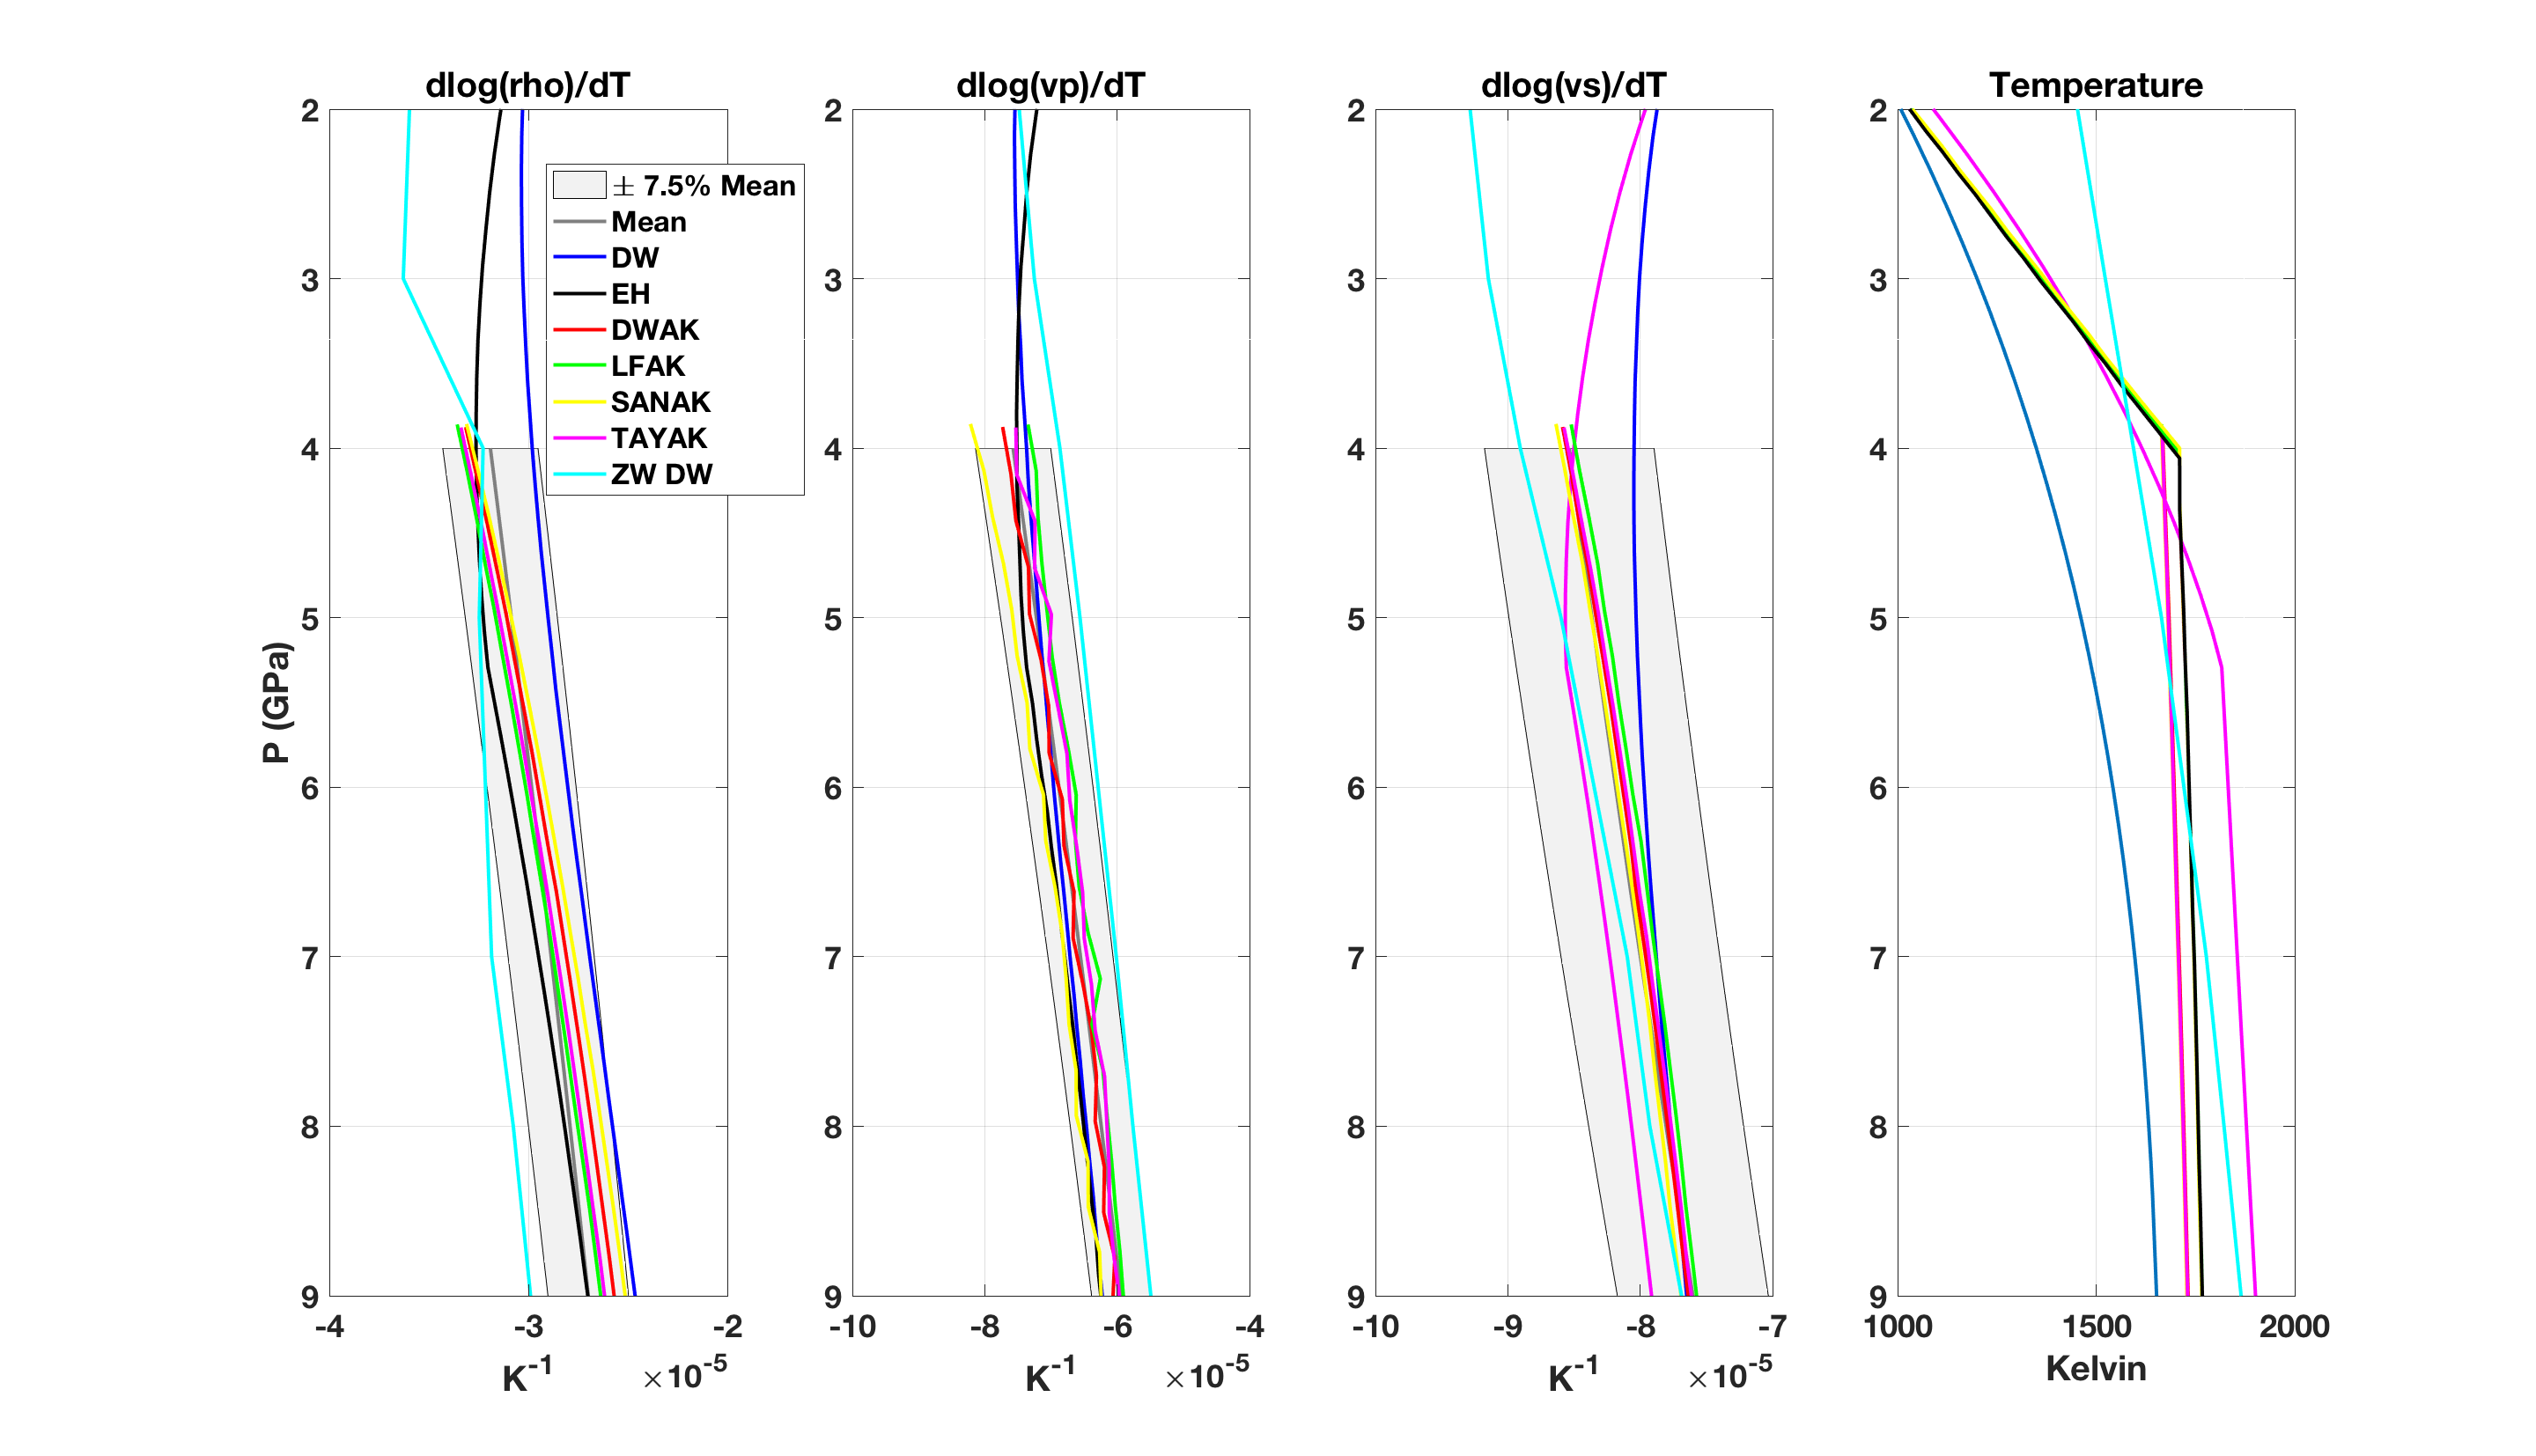
\includegraphics[width=1.0\textwidth]
{figures/Fig20_Interior_updated}
\caption{Temperature dependence of the reference models density and seismic velocities, together with mantle temperature of these models up to 8 MPa (about 600 km depth). These temperature dependencies are computed with a fixed mineralogy, which may be the case in the martian lithosphere. From left to right, the relative density, vp and vs sensitivities and the mantle temperature, at constant pressure. Grey zone is the $\pm$ 7.5\% area with respect to the mean sensitivity models, as defined in text and in Table ~\ref{table:TableEmp}.}
\label{fig:Fig20_Interior.png} 
\end{center}
\end{figure}

\begin{figure}[h!]
\begin{center}
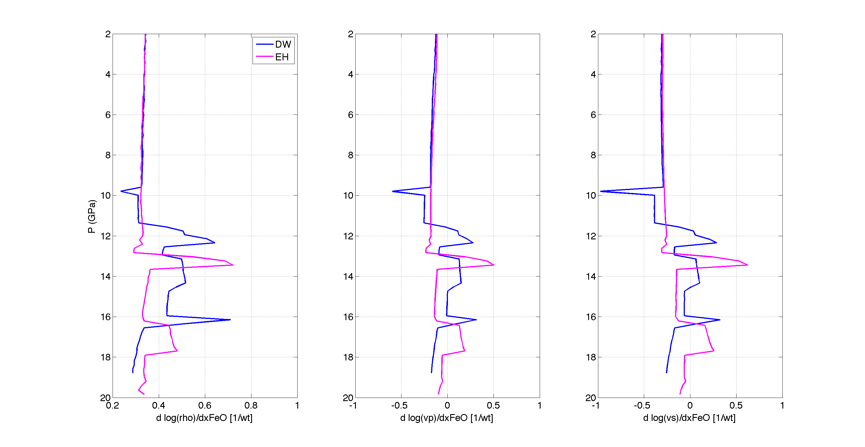
\includegraphics[width=1.0\textwidth]
{figures/Fig3-3-3.png}
\caption{Dependence of DW and EH45 models to FeO content.}
\label{fig:Fig3-3-3.png} 
\end{center}
\end{figure}

As shown in Section 3.1, large temperature variation are expected in the Martian lithosphere, mostly due to the large crustal heating lateral variations and to the large elastic lithosphere thickness, which allows such temperature lateral variation to be maintained over geological times. At 200 km depth, these temperature variations can be $\pm$150$^{\circ}$C for the models with the smallest variations, but can be up to $\pm$535$^{\circ}$C for those with the largest.
As seen above, the temperature sensitivities of both seismic velocities and densities are not strongly dependent on the type of models. We show furthermore that a simple linearized model can therefore parameterize these temperature variations. Figure~\ref{fig:Fig3-3-4.png} shows, for model TAY, the case of the largest temperature differences, i.e. 500$^{\circ}$C at the base of lithosphere for the and compare the non-linear $V_S$ computation $V_S$(T+DT) with the linearized one, $V_S$(T)+$\Delta$T $\times$ d$V_S$/dT. This error is about 10\% of the relative velocity change in the upper mantle, which is less than 0.4\% of the absolute Vs velocity. This error is also 10 times less than the L2 InSight/SEIS mission requirement for the determination of the mantle velocity ($\pm$0.25km/s and therefore about $\pm$6\%) and will therefore be much less than the capability of the mantle structure determination with a single station.

\begin{figure}[h!]
\begin{center}
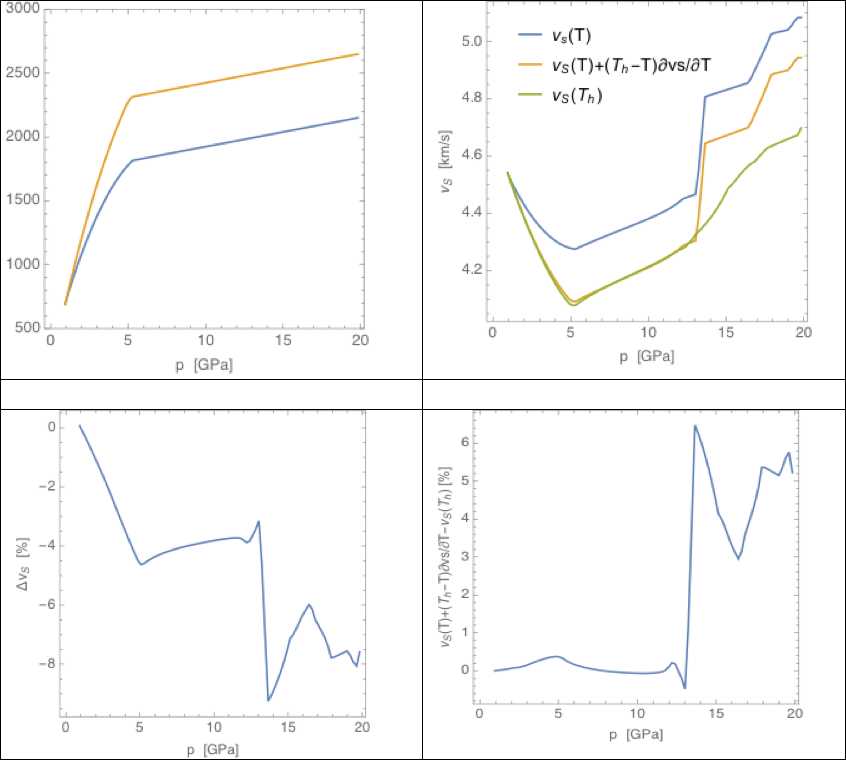
\includegraphics[width=0.8\textwidth]
{figures/Fig3-3-4_v2.png}
\caption{Temperature linearization error. From top left to top right. The two temperature model used and the obtained seismic velocity models, compared with the linearized model. Bottom left to bottom right: relative Vs variation between the two models and the error between the non-linear and linear case, in \%.}
\label{fig:Fig3-3-4.png} 
\end{center}
\end{figure}

\subsubsection{Vp,Vs, density 3D lateral variation}

In the following, we review the present-day possible density and body waves velocity anomalies due to lateral thermal and compositional heterogenetities present within Mars' silicate envelopes. In performing this exercise, one should stress that the presence of that lateral anomalies, even of significant amplitude, does not necessarily imply their unambiguous detection and characterization. This aspect will also be discussed in this section.  

\paragraph{Crustal Heterogenities}

Mars silicate envelope exhibits a variety of ranges for lateral variations in density ($\rho$) and body wave speeds ($v_p$, $v_s$) along its planetary radius, $r$. While the shallow crustal region appears to be characterized by the largest lateral variations, deeper regions are nonetheless also associated with important variations in $\rho$, $v_p$, and $v_s$.

At the surface, the crust can be roughly divided into two/three main domains (e.g., \citep{Solomon1982,Zuber2000,McSween2003}):
\begin{itemize}
  \item The northern lowlands, having a uniformly thin crust ($\sim$30 km on average) mostly composed of andesitic rocks and/or altered basalts.
  \item The southern highlands, consisting of a thick crust ($\sim$60 km on average) mostly composed of basaltic rocks. 
  \item The Tharsis Rise, located at the boundary between these two domains, where intense plume activity formed a thick ($\sim$100 km) basaltic crust.
\end{itemize}


At depth, one can expect these domains to be subdivided into different units, characterized by the following ranges, whose values are mostly inspired by \citet{Mavko2009}: 
\begin{itemize}
	\item Between 0 and 5 km depth, a heterogeneous superficial crust where various types of rocks coexist (sedimentary and igneous), leading to a wide range of densities and seismic velocities, from altered basalts ($\rho$=2700-3100 kg/m$^3$; $v_p$=5-6 km/s; $v_s$=2.8-3.4 km/s) to mudstones, shales, clays, sands and loess ($\rho$=1500-2500 kg/m$^3$; $v_p$=0.5-3.5 km/s; $v_s$=0.2-1.7 km/s). Moreover, different types of anisotropy could further affect the seismic velocities, such as sedimentary or lava flow layering (12-15\% variation), and the presence of wide damage zones surrounding long-term fault networks. Indeed, many studies have shown that damage zones could reduce seismic velocities from 10\% to 50\% depending on the structural maturity of the fault and regardless the geological context (see a compilation on Earth in \citet{Perrin2016}, their table S5). \citet{Cochran2009} also documented seismic velocities reduced by 40-50\% across a fault zone of 1.5 km wide in the Mojave Desert, which can be considered as a good geological analog for Mars (e.g., \citep{Golombek1997,Marlow2008}).
    \item The lithostatic pressure increase could result in a 10-12\% increase in velocities for sandstones between 0 and 50 MPa due to porosity reduction \citep{Han1986}.
    \item Between 5 and 15-20 km depth, an upper crust mostly formed by more differentiated volcanic materials, such as andesite, or altered basaltic rocks ($\rho$=2400-2800 kg/m$^3$; $v_p$=4.5-6 km/s; $v_s$=2.5-3.3 km/s). The variation of seismic velocity can still be affected by the layering of lava flows. However, below 5 km depth, fault damage zones become considerably reduced (e.g., \citep{Ben-Zion2003,Finzi2009,Allam2014} for studies on Earth), therefore limiting the lateral effect on seismic velocities. The gravity being smaller on Mars than on Earth, this depth may be larger than the aforementioned value.
    \item Between 15-20 and 30-100 km depth, a lower crust mainly composed of compacted basalts ($\rho$=2700-3100 kg/m$^3$; $v_p$=5-7.2 km/s; $v_s$=2.8-4 km/s), where various types of seismic anisotropy (lithological, structural, or stress-induced) can possibly occur (yielding an anisotropy up to 15-30\% on Earth, e.g., \citep{Crampin1991,Weiss1999}.
\end{itemize}


Figure~\ref{fig:lateral_lithosphere_anomalies}a-c summarizes the aforementioned plausible ranges of lateral crustal variations in density and body wave speeds.
Note that Mars' deep crustal density range has recently been questioned on the basis of in-situ chemical composition analyses, GRS maps, and SNC meteorites analysis \citep{Baratoux2014}. This has led to a higher range for crustal densities ($\sim$ 3100-3600kg/m$^3$), which may imply a deeper extent of Mars' crust in order to satisfy constraints on the moment of inertia. Although a deep eclogitic root would be gravitationally unstable and more easily prone to delamination, the larger crustal viscosities at such colder depths may efficiently delay in parts delamination processes, depending on the activation energy of the crustal material. For now, we will restrict our expectations to the more conservative estimates displayed in  Figure~\ref{fig:lateral_lithosphere_anomalies}a, however InSight's expected seismic record and heat flux measurements would allow the possibility of a deep ($\sim$ 100-200 km thick) eclogitic root to be tested.

\begin{figure}[h!]
\begin{center}
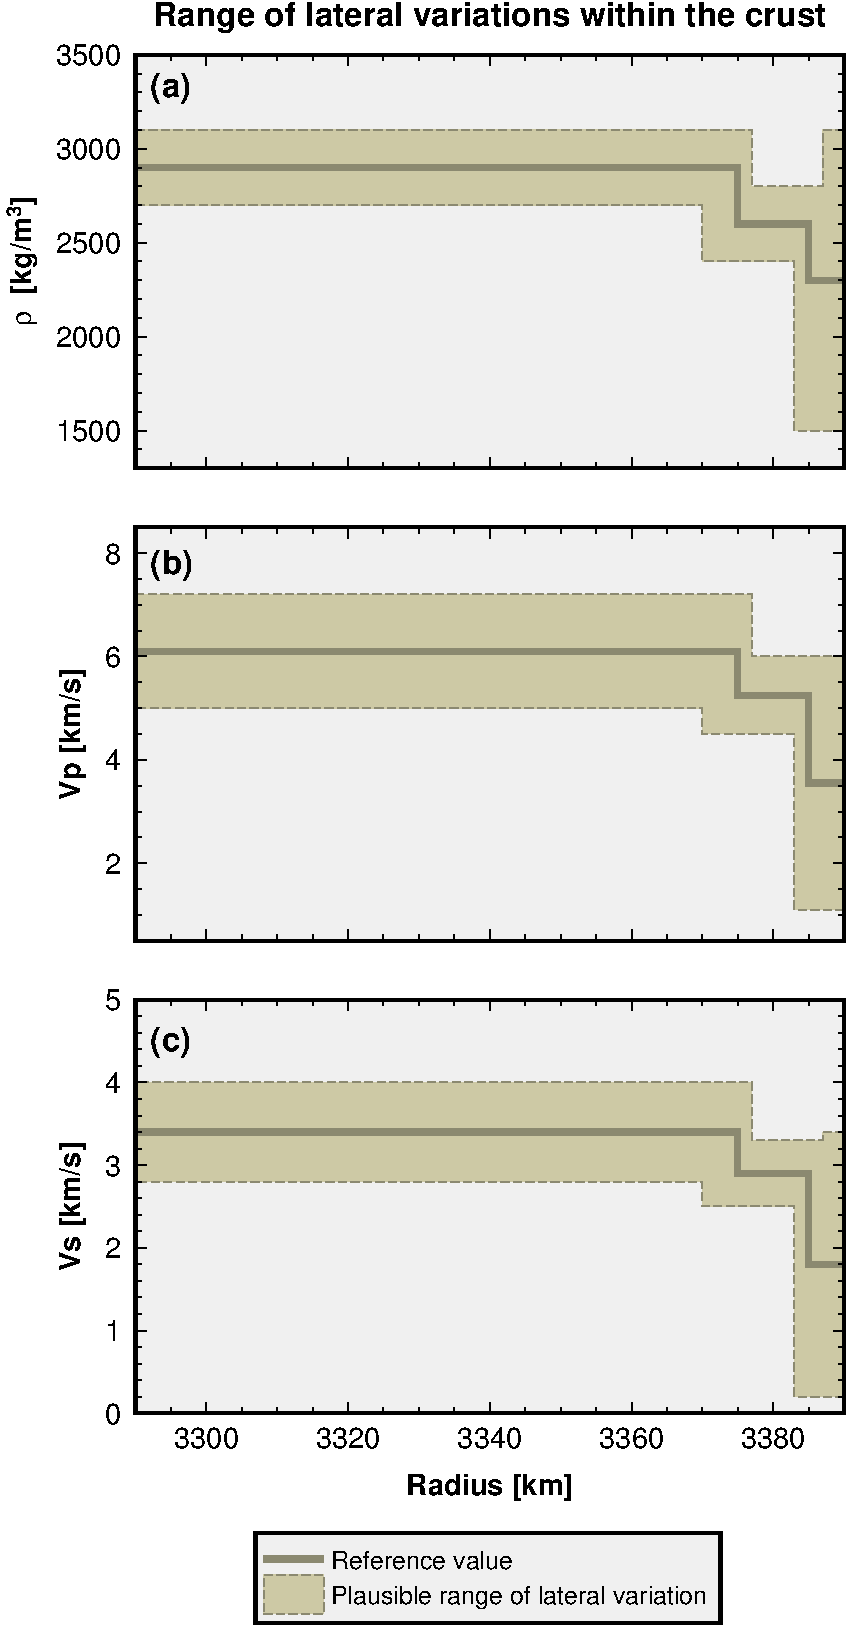
\includegraphics[scale=0.5]
{figures/Lateral_het_crust.pdf}
\caption{Plausible range of lateral crustal variations in density (a), P-wave (b) and S-wave (c) velocities within Martian crust region. See text for further details.}
\label{fig:lateral_lithosphere_anomalies}  
\end{center}
\end{figure}

In addition to lithological/petrological differences, the highlands and the lowlands are also expected 
to exhibit a distinct temperature structure. The southern hemisphere could be more than 300K hotter than the northern hemisphere over depths greater than 250 km, as a result of their different thicknesses and heat-producing element contents, as further discussed below.


\paragraph{Lithosphere and Mantle Heterogeneities}
In the deeper lithospheric region, changes in composition and (P,T) conditions lead to different ranges of lateral variations. The likely convective style of present-day Mars mantle corresponds to a stagnant-lid regime, in which a thick cold and highly viscous lithosphere (i.e., the lid) overlays a convective mantle. Lateral heterogeneities in the lithospheric region may result from variations in the thickness of the crust and the stagnant lid. The latter are mainly controlled by the interplay between rheology, heterogeneous internal heating due to variable enrichment in heat producing elements, and convective processes (e.g., \citep{Plesa2016} and references therein; \citep{Thiriet2018}). These constraints can be incorporated into numerical models of solid-state convection with temperature-dependent viscosity, conducted in spherical geometry. In this context, we have considered two end-member cases. 
One reference model discussed in section~\ref{ref_temp}, having a strong pressure-dependence of viscosity, with an activation volume of 10 cm$^3$/mol, and matching a number of observational constraints (past and present elastic thicknesses, volcanism etc., see section 3.1). 
We also considered a second case, which only differs from the reference model by the fact that  viscosity does not depend on pressure. This model produces small temperature variations in the convecting mantle, comparable to the cold end-member case considered in section ~\ref{ref_temp} and Table~\ref{table:end_member_ref_models}.
Lateral anomalies in density and body-waves speeds can then be estimated along the planetary radius using conversion coefficients $\partial \ln\rho/\partial T$, $\partial \ln v_p/\partial T$, $\partial \ln  v_s/\partial T$ derived from Gibbs free-energy minimization, and the latter are described in section 3.2. Variations in crustal and lithosphere thickness yield important peak-to-peak temperature anomalies. Their plausible range are shown in Figure~\ref{fig:Fig4.png} and summarized in Table~\ref{table:T_induced_variations} for two extreme temperature models (high and  low $\delta T$) and for the reference model described in section~\ref{ref_temp} (Table~\ref{table:end_member_ref_models}). 

\begin{table}[h!]
\centering
\caption{Plausible ranges of lateral variations in temperature, and temperature-induced density and seismic velocity variations. Sensitivities range are set to -2.5/-3.5 10$^{-4}$ K$^{-1}$, -6.5/-7.5 10$^{-4}$ K$^{-1}$, -8/-9 10$^{-4}$ K$^{-1}$ for density, $v_p$ and $v_s$ respectively. The three temperature models are those of section~\ref{ref_temp} .}
\begin{tabular}{l|lllll}
                            & Min. T& Max. T & $\delta\rho/\rho$   & $\delta v_p$/$v_p$ & $\delta v_s$/$v_s$        \\ \hline
Low $\delta T$ Model        & 1016  & 1316   & 0.8/1.1\%      & 2/2.3\%       & 2.4/2.7\% \\
Reference $\delta T$ Model  & 791   & 1795   & 2.5/3.5\%      & 6.5/7.5\%     & 8/9\%     \\
High $\delta T$ Model       & 629   & 1700   & 2.7/3.7\%      & 7/8\%         & 8.6/9.6\%
\end{tabular}
\label{table:T_induced_variations}

\end{table}

Such variations in crustal and lithospheric thicknesses yield important peak-to-peak anomalies $\delta \rho$=2-3.5\%, $\delta  v_p$=6-8\%, $\delta  v_s$=8-10\% for the reference and high $\delta$T models.  These are also imaged in Figures~\ref{fig:lateral_mantle_anomalies}a-c, which show that lateral variations in density and body wave speeds are more pronounced for the case with pressure-dependent viscosity, as it generates larger temperature variations that erode the cold lid more efficiently.

\begin{figure}[hp!]
\begin{center}
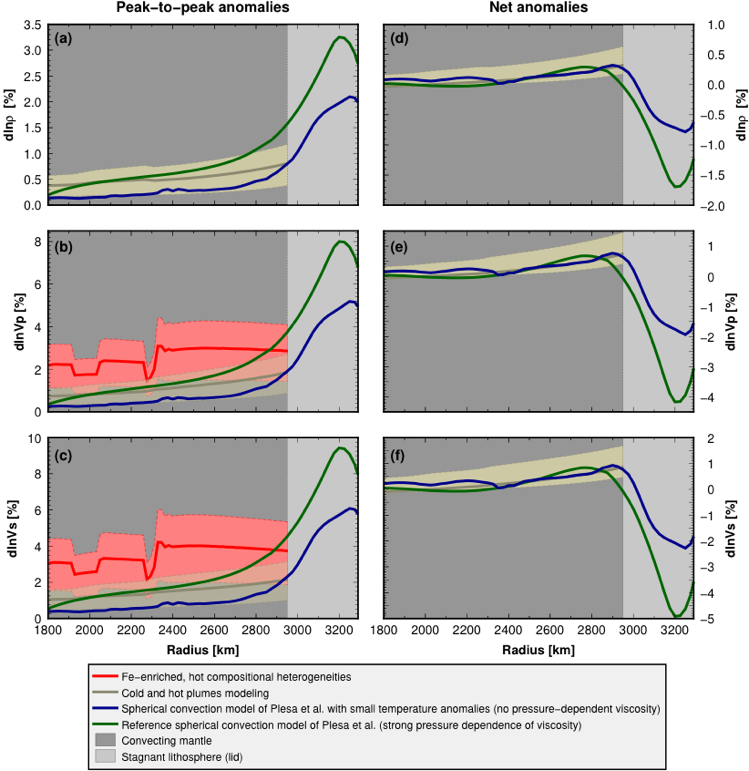
\includegraphics[width=1.0\textwidth]
{figures/Fig3-3-3-3.png}
\caption{ Left (a-c): peak-to-peak lateral anomaly profiles for density (top), P-wave speed (middle), and S-wave speed (bottom) as a function of Mars radius, $r$. The beige colored area corresponds to the contribution of cold and hot axisymmetric plume conduits, obtained from numerical modeling. This area is bounded by two extreme cases (dashed brown curves). The lower bound corresponds to the following governing parameters: $Ra=10^5$, $E$=540 kJ/mol, and temperature contrast across the lower thermal boundary layer $\delta_{\rm TBL}$=50 K. The upper bound corresponds to $Ra=10^7$, $E$=200 kJ/mol, $\delta_{\rm TBL}$=100 K. An intermediate case is shown (thick brown curve) for $Ra=10^6$, $E$=300 kJ/mol, $\delta_{\rm TBL}$=100 K. The anomalies derived from the thermal structure of two spherical thermal convection models are also shown: a case with no pressure dependence of viscosity (blue curves), and yielding the smallest temperature anomalies, and a case with strong pressure-dependent viscosity (green curves). The latter model, described in section 3.1, explains best observational constraints. Anomalies associated with the presence of purely hotter and denser (Fe-enriched) compositional heterogeneities for a range of compositional density contrasts 0.5-1.5\% (light red area bounded by dashed red curves for $\delta \rho_c$/$\rho$=0.5\% and $\delta \rho_c$/$\rho$=1.5\%). The case for $\delta \rho_c$/$\rho$=1\% is illustrated with the thick red curve. Right (d-f): net anomalies resulting from summing the anomalies associated with cold and hot material, which are of opposite sign. These correspond to the same models considered in (a-c), with the exception of the anomalies associated with compositional heterogeneities. See text for further details.}
\label{fig:lateral_mantle_anomalies} 
\end{center}
\end{figure}

The largest shallow temperature variations are however expected to be localized beneath Tharsis and Hellas, and will be detected only for rays passing through. Figure~\ref{fig:Fig3-3-3-2.png} provides, for the three proposed temperature models shown in Table~\ref{table:end_member_ref_models}, the cumulative curve of area percentage at a given temperature at 200km depth.  For the reference model, temperature varies by somewhat less than 300K across 80\% of the surface for the nominal case, reducing the  $v_s$ seismic velocity lateral variations to less than 3\% peak-to-peak, which is  about half the L2 InSight/SEIS mission requirement for the determination of the mantle velocity ($\pm$0.25km/s, therefore, about $\pm$6\%).

\begin{figure}[h!]
\begin{center}
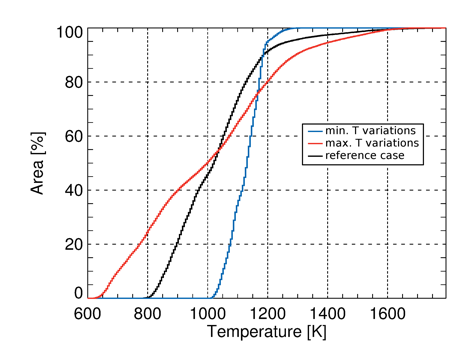
\includegraphics[scale=0.95]
{figures/Fig3-3-3-2.png}
\caption{Cumulative histogram showing the fraction of the surface of Mars at 200km depth where the temperature lies below a given value. The three lines correspond to the three models described in section~\ref{ref_temp}.}
\label{fig:Fig3-3-3-2.png} 
\end{center}
\end{figure}

At greater depths, lateral heterogeneities in present-day Mars mantle most likely result from solid-state convective processes. In the simplest case of purely thermal convection, temperature anomalies, $\delta T$, result from hot upwelling and cold downwelling plume conduits originating from core-mantle, and surface thermal boundary layers (TBL), respectively. To first-order, plumes are axially symmetric objects whose radius $R_p$ broadens with the plume height, $h_p$, as a result of thermal diffusion. The temperature anomaly is maximum along the plume centerline, and decreases away from it. Plume broadening also results in a progressive decrease of the amplitude of thermal anomalies between the plume and its surroundings. These characteristics were predicted by theory \citep{Batchelor1954,Whittaker2006} and were confirmed by laboratory and numerical experiments (\citep{Davaille2011,VanKeken2013}, and references therein). These studies have shown that $R_p \sim (h_p-h')^{1/2} Ra^{-\beta}$, and that the plume centerline temperature $T_c \sim 1/(h^*+h_p) \sim \delta T$, where $Ra$ is the effective Rayleigh number expressing the convective vigor of the mantle, and $\beta \cong $0.2 \citep{Lithgow-Bertelloni2001} . The functions $h^*$ and $h'$ depend on $Ra$, and on the viscosity contrast across active (i.e., mobile) parts of the TBLs, $\Delta \eta$. The latter differ in cold and hot TBLs due to the temperature dependence of viscosity through an activation energy, $E$ (e.g., \citep{Karato1993}), and due to the different amplitudes of temperature variations, $\delta_{\rm TBL}$, across the cold and hot TBL, implying that cold and hot Martian plumes have likely different strengths. The above relationships indicate that the main governing parameters for the temperature anomalies associated with plumes are $Ra$ and $E$, $\delta_{\rm TBL}$ (or equivalently $\Delta \eta$), whom values remain poorly constrained. We computed temperature anomalies associated with cold and hot plumes using high-resolution finite-volume discretization of the Navier-Stokes and the conservation of internal energy equations in axi-symmetric geometry, with temperature-dependent viscosity, under the infinite Prandtl number and Boussinesq approximations \citep{Samuel2012}. 

With the knowledge of plume thermal structure, lateral anomalies in density, $v_p$, and $v_s$ can be estimated along the planetary radius using conversion coefficients, as previously explained. The obtained values for $v_p$ and $v_s$ anomalies are averaged over spherical regions with a radius of 15 km and 10 km corresponding to typical sizes of Fresnel zones for P and S waves, respectively.

It should be noted that phase transitions occurring within Mars' mantle (e.g., olivine-wadsleyite and wadsleyite-ringwoodite) could produce peak values in relevant derivatives of thermoelastic properties \citep{Stixrude2007}. The details  depend on the details of the specifics of the compositional models Figure~\ref{fig:Fig_dT.png} and the iron content Figure~\ref{fig:Fig_dFeO.png}. These would result in possibly large amplitude peaks in $d\ln \rho$, $d\ln v_p$, $d\ln v_s$. However, the amplitude of such peaks depends on poorly constrained values of physical parameters such as the Clapeyron slope and the pressure range over which the phase transitions occur. In addition, these peaks are likely to be very narrow. For these reasons, the conversion coefficients $\partial \ln\rho/\partial T$, $\partial \ln v_p/\partial T$, and $\partial \ln v_s/\partial T$ we used to infer the anomalies displayed in Figure~\ref{fig:lateral_mantle_anomalies} correspond to isomorphic contributions. 



Figure~\ref{fig:lateral_mantle_anomalies}a-c shows the plausible range of peak-to-peak (i.e., from hot to cold plumes) lateral anomaly profiles along $r$ (inferred from the plausible ranges for $Ra=10^5-10^7$, $\delta_{\rm TBL}$=50-100 K for the bottom TBL, $\delta_{\rm TBL}$=100-200 K for the (mobile) part of the upper TBL, and $E$=200-540 kJ/mol). Upper and lower TBLs were not included since purely lateral thermal anomalies would vanish in these regions. The median values range between 0.5\% and 1\% $\pm$ 1\%. $v_s$ anomalies are more pronounced than $v_p$, due to the higher sensitivity to temperature of the shear modulus compared to that of the bulk modulus. The increase of lateral anomalies with increasing $r$ primarily results from the pressure-dependence of physical properties (bulk and shear moduli, $\rho$, and their temperature dependence), and secondarily from the asymmetry between stronger cold and weaker hot plumes at a given $Ra$ value, leading to an increase in peak-to-peak temperature anomalies with increasing $r$. 

This simple plume modeling approach does not account for additional potential complexities of Martian mantle dynamics such as plume interactions, pressure-dependent viscosity \citep{Leng&zhong2008}, the presence of a heterogeneous crust of variable thickness, phase changes, or sphericity. Such complexities may in particular enhance the top-bottom asymmetry between upwellings and downwellings or could affect the thermal structure of plume conduits. To assess such influences we have considered the thermal structure derived from the two models in spherical geometry mentioned above (the blue and green curves in Figure~\ref{fig:lateral_mantle_anomalies}). The model with no pressure dependence of viscosity (blue curves in Figure~\ref{fig:lateral_mantle_anomalies}a-c) agrees well with the lowest end of lateral anomalies inferred from the plume modeling. The second model with strong pressure-dependence of the viscosity exhibits peak-to-peak anomalies in the lowermost mantle that are smaller than the plausible range covered by the plume model (green curves in Figure~\ref{fig:lateral_mantle_anomalies}a-c). However, the more pronounced top-bottom asymmetry (enhanced by pressure-dependent viscosity) leads to an increase in anomalies with $r$, to values larger than the plume models at shallower depths. 

The possibility of thermo-chemical convection suggested by the identification of geochemical reservoirs within Mars mantle through the analysis of the SNC meteorites \citep{Debaille2007} should also be considered. In this case, the survival of compositional heterogeneities in a convective mantle most likely occurs through the presence of denser (possibly Fe-enriched) material, which gradually heats up, as it does not participate in convection \citep{Samuel2003}. Such a hot and denser material must remain sufficiently stable to prevent convective mixing, and sufficiently buoyant to be sampled and brought to the surface by upwelling plumes, as suggested by the analysis of the SNC meteorites. This can occur provided that the compositional density contrasts and thermal density contrasts remain comparable: $\delta \rho_c/\rho \sim \alpha(r)\delta T(r)$ \citep{LeBars2004}. This constraint yields a rough estimate for $\delta T(r)$, assuming that the other parameters are reasonably well known. We used $\alpha(r)$ from DW, see section 3.4.2. Numerical experiments \citep{Tosi2013} have suggested that a plausible range for  $\delta \rho_c/\rho$ would be about 0.5\%-1.5\%. Such a range is considered in Figure~\ref{fig:lateral_mantle_anomalies}a-c, and yields the largest peak-to-peak anomalies in the convective mantle, despite the fact that cold plume contributions were not even considered for this case. Note that $v_p$ and $v_s$ anomalies also account for the Fe-enrichment assumed for the denser material, but this influence is minor compared to the temperature effect. Although their size, shape and volume are largely unconstrained, such hypothetical compositional heterogeneities could significantly contribute to lateral heterogeneities within the deep Martian mantle.

Finally, as pointed out earlier, the presence of lateral anomalies within Mars' mantle can be clouded in a number of ways. 
A good example of the difficulty in detecting and characterizing lateral seismic anomalies is the Earth's mantle, where density and seismic velocity anomalies of comparable or larger amplitudes than those discussed in this section remain difficult to image. Indeed, despite an obviously much denser seismic array, and vast amounts of high-quality data, the seismic detection of mantle plume anomalies on Earth remains debated (\citep{Montelli2004,VanderHilst2006} and references therein), and in the best case is prone to trade-offs between the size of the anomalies and their amplitude \citep{French2014}. 
The difficulty in detecting lateral anomalies could result from a number of processes, such as the sampling of anomalies of smaller size than the wavelength of the seismic waves, the presence of sharp velocity gradients along interfaces with a possibly complex topology triggering multiple reflections, the development of shadow  zones associated with slow velocity anomalies, etc.

In addition, the opposite signs of $\partial \ln\rho / \partial T$, $\partial \ln v_p / \partial T$, $\partial \ln v_s/ \partial T$ associated with cold and hot anomalies may, to some extent, cancel out each other, as seismic waves integrate positive and negative anomalies along their paths. This last possibility is illustrated in Figure~\ref{fig:lateral_mantle_anomalies}d-f where the resulting net sum of hot and cold anomalies shown are two to four times smaller than peak-to-peak anomalies (Figure~\ref{fig:lateral_mantle_anomalies}a-c). While this outcome depends on a number of unknown parameters such as the distribution of hot and cold anomalies, or source locations, it underlines the fact that canceling lateral anomalies may hinder the presence of heterogeneities of much larger amplitude.
More generally, it is likely that the SEIS experiment would only detect a smaller fraction of the anomalies predicted in Figures~\ref{fig:lateral_lithosphere_anomalies} and Figures~\ref{fig:lateral_mantle_anomalies}a-c.
However, the expected important temperature differences over a significant lithospheric depth range between the southern and the northern hemisphere would be sufficiently large to allow for a seismic detection by surface waves, provided a favorable location of the seismic sources \citep{Panning2016}.
The seismic detection of the north-south dichotomy (or even its non-detection) by SEIS would provide important information regarding the present-day thermal state or Mars, and/or the rheological properties of its silicate envelope. Additionally, the IFG will provide magnetic field measurements at the Martian surface. If separable from fluctuations due to the lander, periodic variations in the Martian magnetic field will be monitored and recorded. Such variations have already been observed in orbit (Langlais et al., 2017; Mittelholz et al., 2017). The analysis of these measurements may provide more robust constraints on the electrical conductivity profile at depth, which, when combined with velocity profiles derived from SEIS, should improve models of the interior of Mars.


\begin{figure}[h!]
\begin{center}
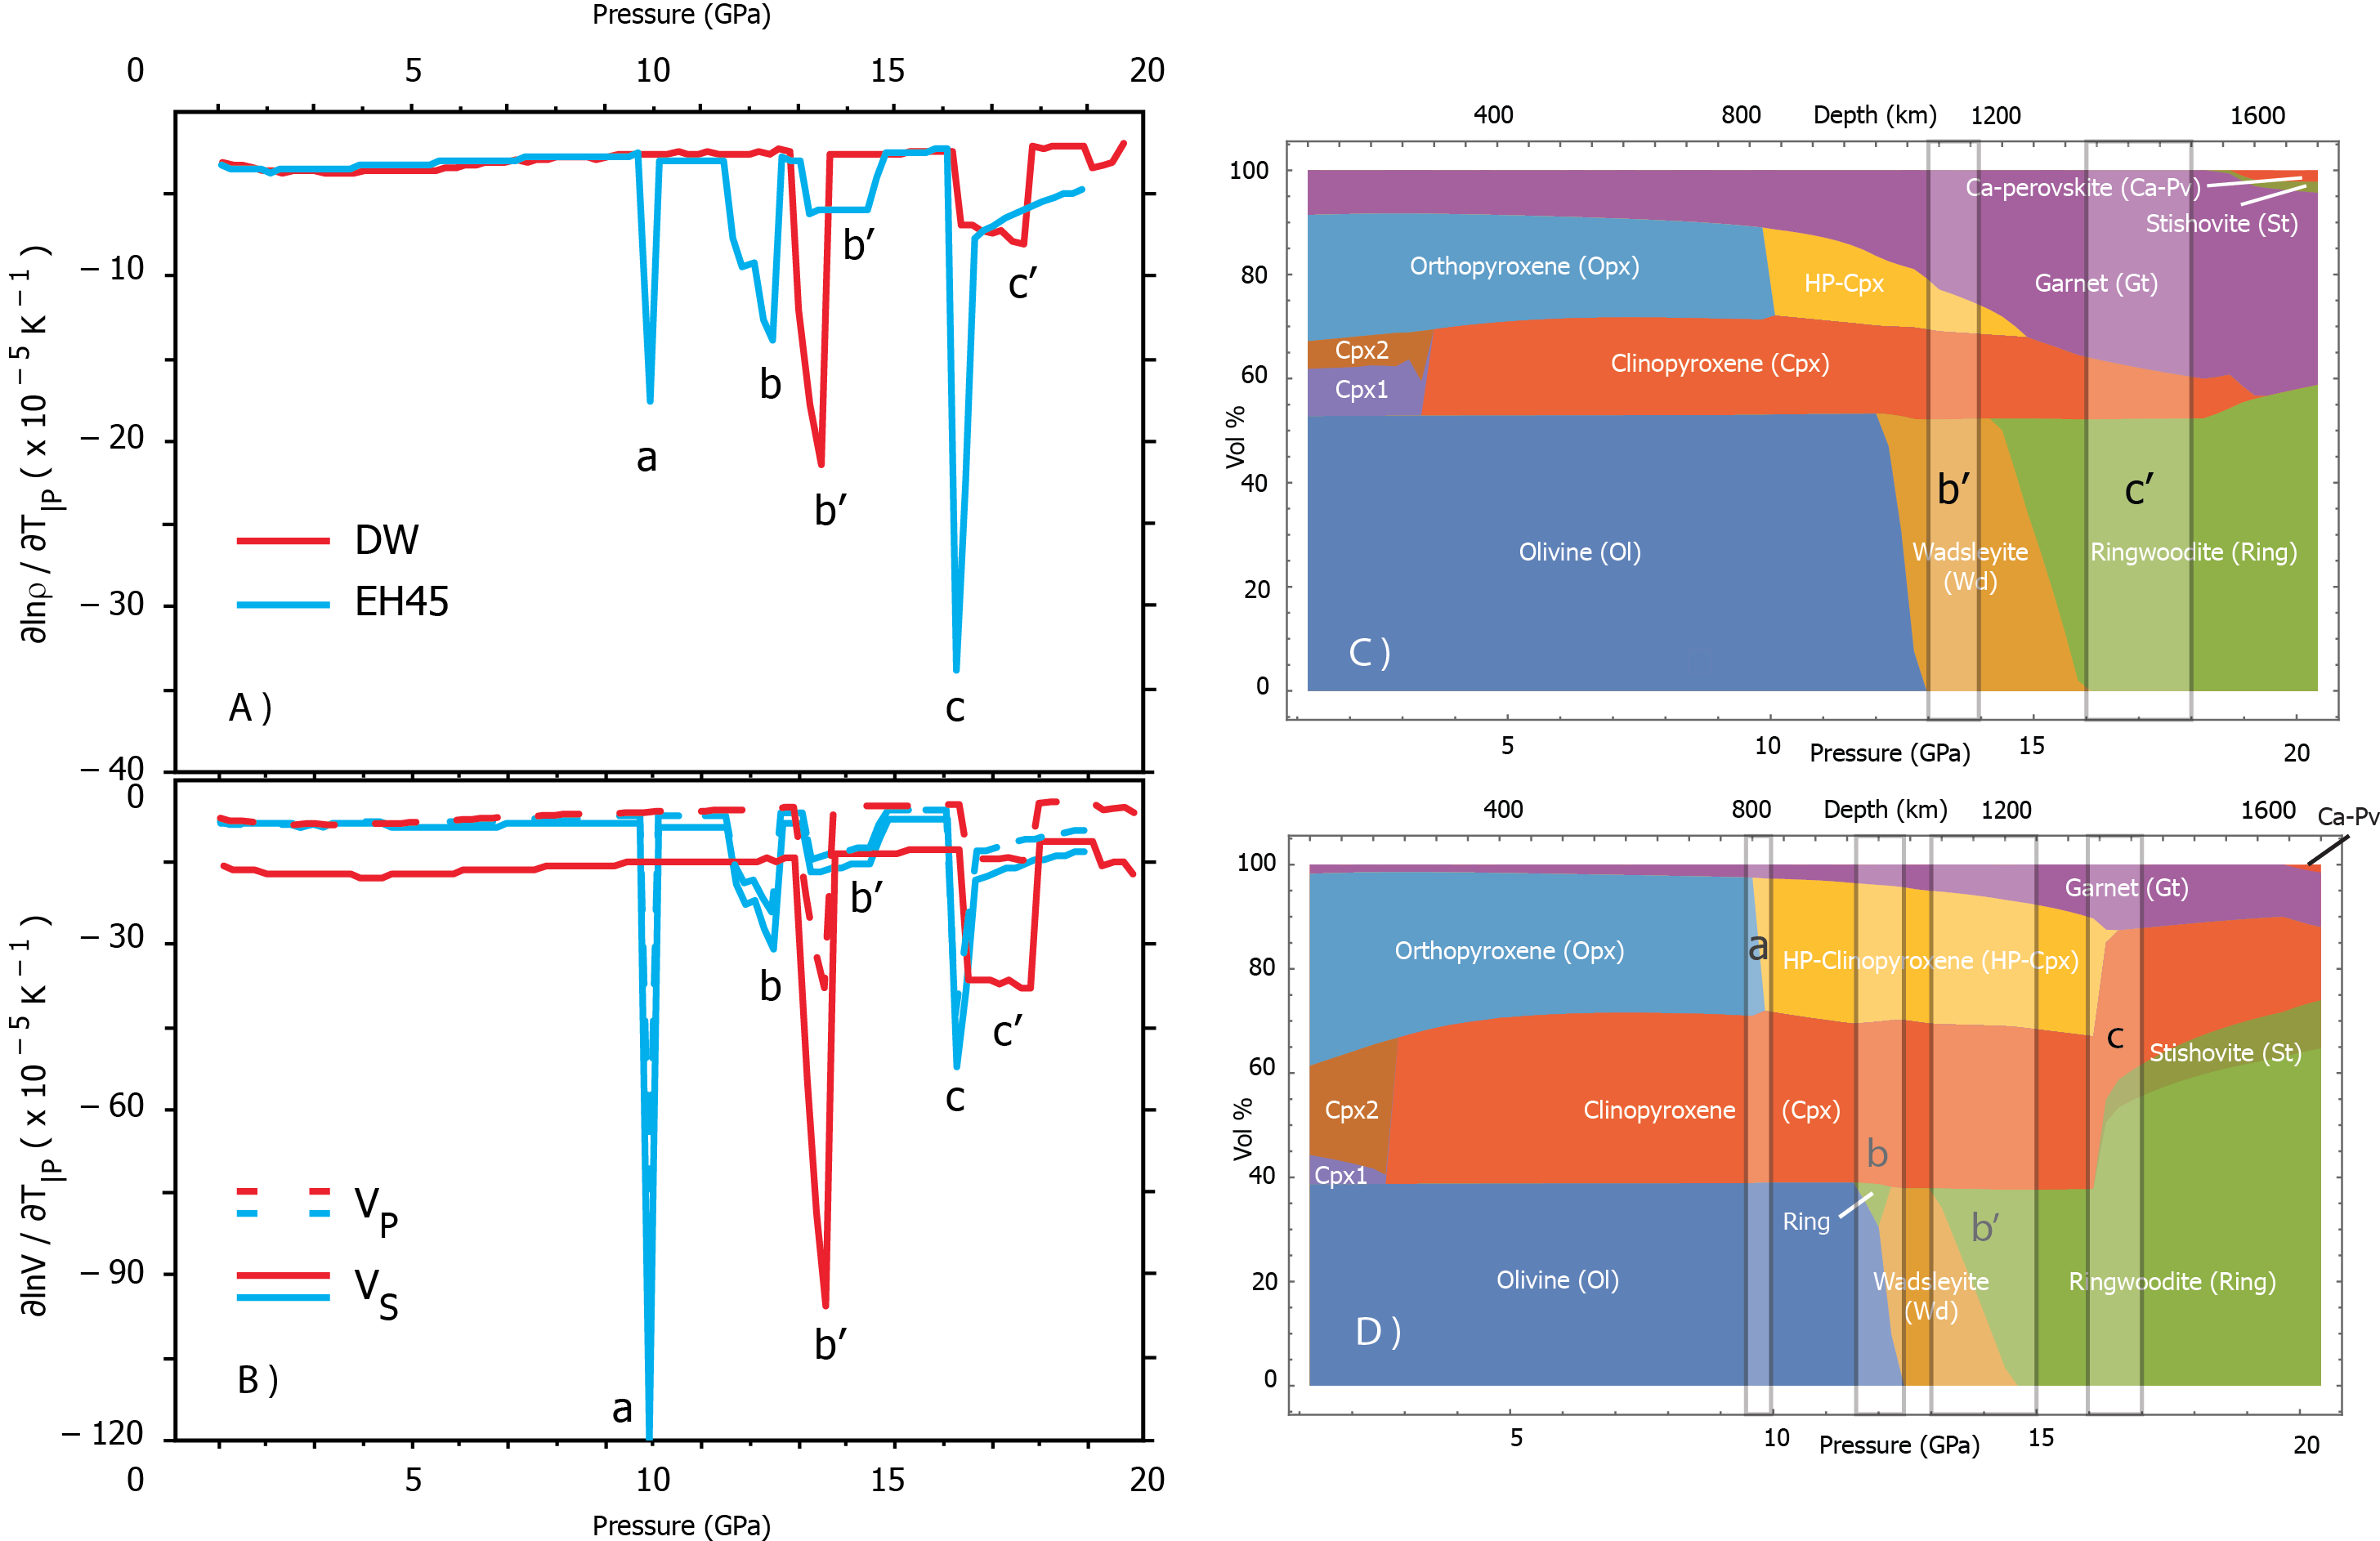
\includegraphics[width=1.0\textwidth]
{figures/Fig_dT.png}
\caption{Two examples of the temperature dependence of Mars' mantle models. DW : olivine-rich composition of \citet{Dreibus1984} revised in \citep{Taylor2013}; EH45 : pyroxene-rich composition of \citet{Sanloup1999}. In the left panels the sensitivity of the density (A) and seismic velocities (B) to temperature perturbations are plotted as a function of pressure. The labeled peaks are induced by the mineralogical transformations displayed in the right panels for the DW (C), and EH45 (D) compositions.}
\label{fig:Fig_dT.png} 
\end{center}
\end{figure}

\newpage
\begin{figure}[!h]
\begin{center}
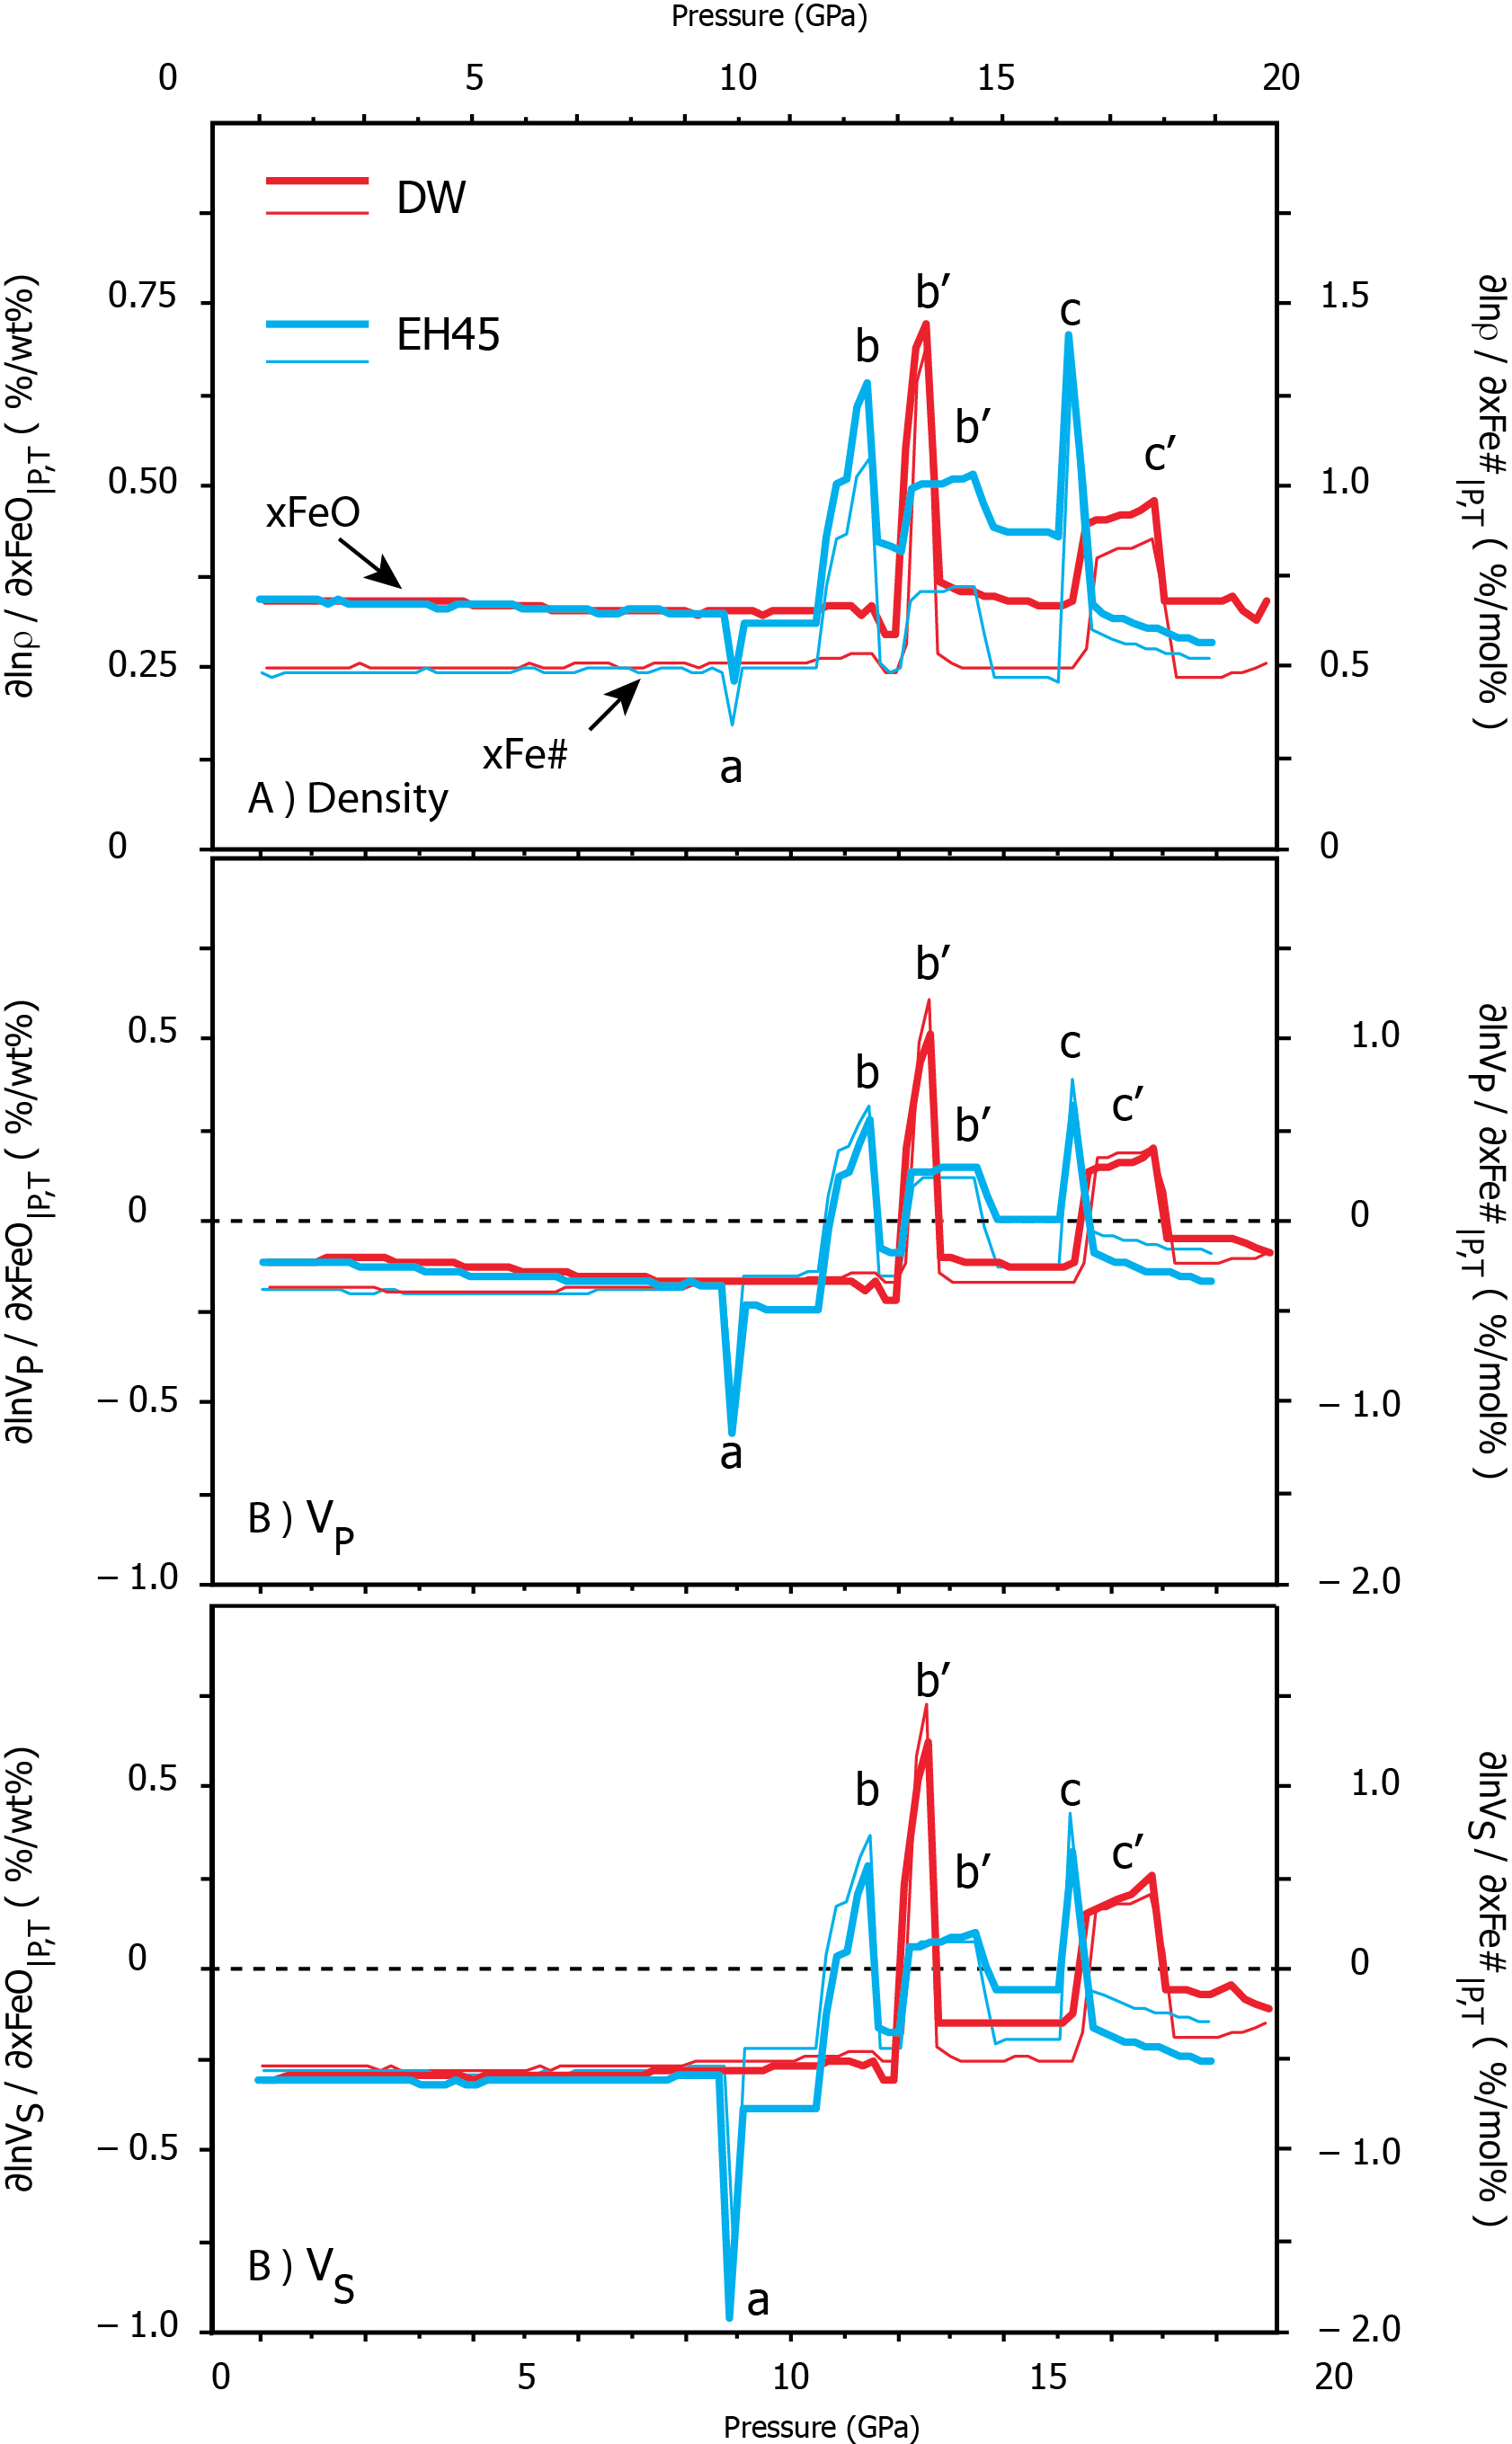
\includegraphics[width=1.0\textwidth]
{figures/Fig_dFeO.png}
\caption{Same as Figure~\ref{fig:Fig_dT.png} for the dependence on the FeO content. Heavy curves and left y-axis refer to a bulk variation of the FeO content. Thin curves and right y-axis refer to a molar Fe\# variation within the \ce{[Mg_xFe_{(1-x)}]O} compound. The labeled peaks refer to the mineralogical transformations illustrated in Figure~\ref{fig:Fig_dT.png}C and D.}
\label{fig:Fig_dFeO.png} 
\end{center}
\end{figure}
